\section{Experiments} \label{sec: experiments}

In this section, the proposed IMF compression algorithm is assessed against baseline codecs following the implementation details. Moreover, ablation studies are presented to investigate the effect of different parameters in IMF.

\subsection{Rate-Distortion Performance} \label{sec: rate_distortion_performance}
In this section, we plot the PSNR-bpp curves for each algorithm to compare their compression performance. The corresponding SSIM-bpp curves are postponed to the appendix.
In the figures, for each compressed image, bpp and PSNR values are calculated. Then, for each compression method, PSNR values are interpolated linearly in some fixed bpp values in the range $(0.05, 0.5)$. 
In the following plots, the average performance over all images is reported, along with the standard deviation which is presented as shadows.
For the missing bpp values, the average is extrapolated quadratically and is shown by dashed lines.

In Figure \ref{fig: compression_performance_kodak_clic}, the compression performance on the Kodak and CLIC datasets is reported. 
In this figure, the proposed IMF compression algorithm outperforms the SVD-based compression, which can be attributed to the quantization errors that SVD is prone to during encoding and decoding, deteriorating its performance. In this view, the quantization-free property of IMF effectively guarantees higher performance in different bpp values.
It is also evident that the IMF compression algorithm outperforms JPEG in low bpp values.
\begin{figure}[t]
	\centering
	\begin{subfigure}{.45\textwidth}
		\centering
		\includegraphics[width=.95\textwidth]{figures/comparison_kodak_psnr.pdf}
		\caption{performance on Kodak}
		\label{fig: psnr-vs-bpp kodak}
	\end{subfigure}%
	\begin{subfigure}{.45\textwidth}
		\centering
		\includegraphics[width=.95\textwidth]{figures/comparison_clic_psnr.pdf}
		\caption{performance on CLIC}
		\label{fig: psnr-vs-bpp clic}
	\end{subfigure}
	\caption{Performance comparison of JPEG, SVD, and IMF compression algorithms on Kodak and CLIC. 
    % The average PSNR of compressed images is reported in different bpps values in the range $[0.05,0.5]$.
    }
	\label{fig: compression_performance_kodak_clic}
\end{figure}

\subsection{Qualitative Performance}
% The first channels of factor maps $\bm{\mathcal{U}}_{Y}, \bm{\mathcal{U}}_{C_B}$ and $\bm{\mathcal{V}}_{Y}$ defined in \eqref{eq: reshaped factors} are depicted in Figure \ref{fig: imf_components} for an image selected from the Kodak dataset. 
% It is evident that each channel of factor maps can be treated as an 8-bit grayscale image in the lossless compression stage of the encoder. The channels with higher energy maintain the overall texture of the original image, while channels with lower energy focus more on subtle changes. 

The qualitative comparison is made in Figure \ref{fig:qualitative_comparison} where the compressed images by different algorithms are shown in different bpp values.
As can be seen, the proposed IMF compression algorithm is capable of maintaining quality compressed images in bpp values as low as $0.15$, outperforming JPEG and SVD-based methods which suffer from maintaining balanced colors in low bpp values. The artifacts in color produced by JPEG are visible in both example images.

\begin{figure}[t]
	\centering
	\begin{subfigure}{.23\textwidth}
		\centering
		\text{\small Original image}
		\includegraphics[trim=1.7cm 1.5cm 1.7cm 1.7cm, clip, width=1\textwidth]{figures/kodim21_original.pdf}
		\vspace{-20pt}
		\caption*{}
	\end{subfigure}%
	\begin{subfigure}{.23\textwidth}
		\centering
		\text{\small JPEG}
		\includegraphics[trim=1.7cm 1.5cm 1.7cm 1.7cm, clip, width=1\textwidth]{figures/kodim21_JPEG_bpp_0.293.pdf}
		\vspace{-20pt}
		\caption*{\tiny \textbf{PSNR: 25.40dB ~ bpp: 0.29}}
	\end{subfigure}
	\begin{subfigure}{.23\textwidth}
		\centering
		\text{\small SVD}
		\includegraphics[trim=1.7cm 1.5cm 1.7cm 1.7cm, clip, width=1\textwidth]{figures/kodim21_SVD_bpp_0.315.pdf}
		\vspace{-20pt}
		\caption*{\tiny \textbf{PSNR: 23.62dB ~ bpp: 0.31}}
	\end{subfigure}
	\begin{subfigure}{.23\textwidth}
		\centering
		\text{\small IMF}
		\includegraphics[trim=1.7cm 1.5cm 1.7cm 1.7cm, clip, width=1\textwidth]{figures/kodim21_IMF_bpp_0.305.pdf}
		\vspace{-20pt}
		\caption*{\tiny \textbf{PSNR: 25.71dB ~ bpp: 0.30}}
	\end{subfigure}
	
	
	\begin{subfigure}{.23\textwidth}
		\centering
		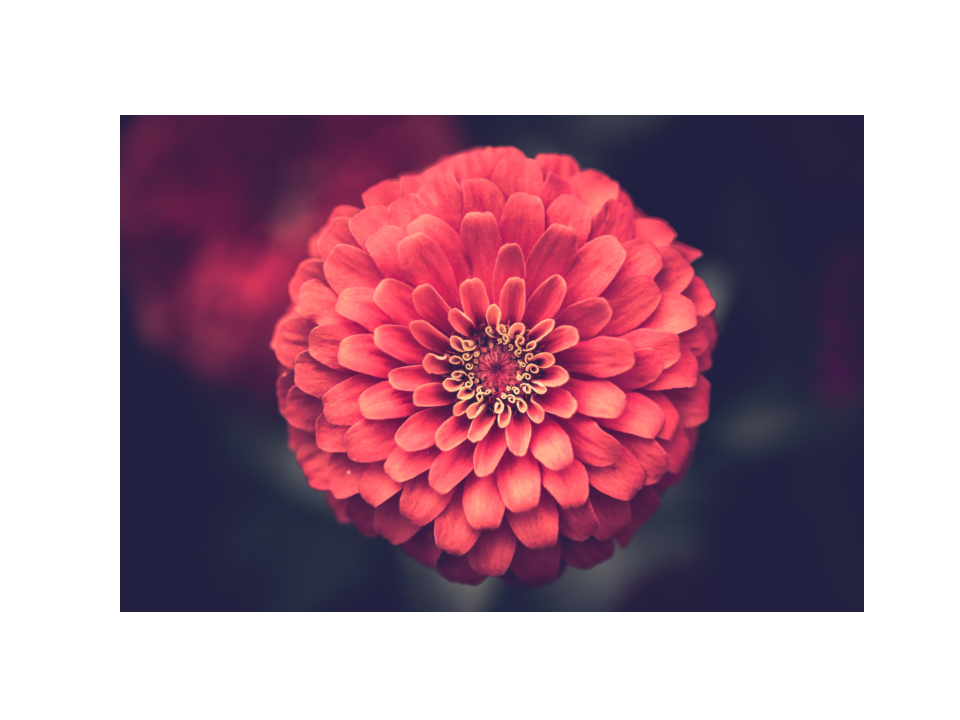
\includegraphics[trim=1.7cm 1.5cm 1.7cm 1.7cm, clip, width=1\textwidth]{figures/clic_flower_original.pdf}
		\vspace{-20pt}
		\caption*{}
	\end{subfigure}%
	\begin{subfigure}{.23\textwidth}
		\centering
		\includegraphics[trim=1.7cm 1.5cm 1.7cm 1.7cm, clip, width=1\textwidth]{figures/clic_flower_JPEG_bpp_0.137.pdf}
		\vspace{-20pt}
		\caption*{\tiny \textbf{PSNR: 22.65dB ~ bpp: 0.13}}
	\end{subfigure}
	\begin{subfigure}{.23\textwidth}
		\centering
		\includegraphics[trim=1.7cm 1.5cm 1.7cm 1.7cm, clip, width=1\textwidth]{figures/clic_flower_SVD_bpp_0.123.pdf}
		\vspace{-20pt}
		\caption*{\tiny \textbf{PSNR: 26.85dB ~ bpp: 0.12}}
	\end{subfigure}
	\begin{subfigure}{.23\textwidth}
		\centering
		\includegraphics[trim=1.7cm 1.5cm 1.7cm 1.7cm, clip, width=1\textwidth]{figures/clic_flower_IMF - YCbCr_bpp_0.108.pdf}
		\vspace{-20pt}
		\caption*{\tiny \textbf{PSNR: 31.73dB ~ bpp: 0.10}}
	\end{subfigure}
	
	\caption{Qualitative performance comparison on an image from Kodak (top row) and CLIC (bottom row).}
	\label{fig:qualitative_comparison}
\end{figure}


\subsection{ImageNet Classification Performance} \label{sec: imagenet Classification Performance}
As another criterion, we investigate the performance of an image classifier on the images compressed by different compression algorithms. 
This criterion focuses on the capability of different compression methods to preserve the visual semantic information in each image.
Furthermore, it highlights the importance of image compression where various vision tasks such as classification---rather than maintaining the perceived image quality---are the main objective, while keeping the requirement of resources such as memory, communication bandwidth, computation power, latency budget, etc. as limited as possible.
ImageNet \cite{deng2009imagenet} validation set, containing 50000 images with a resolution of $224 \times 224$ in 1000 classes, is considered in this classification task done by a ResNet-50 classifier \cite{he2016deep}, pre-trained on the original ImageNet dataset.
The classification performance comparison is made in Figure \ref{fig: imagenet_classification}. 
The results suggest that IMF leads to more than a $25\%$ relative improvement in top-1 accuracy over JPEG at the low bitrate of 0.23 bpp and reaches top-5 accuracy of more than $70\%$ at the bpp value of 0.2. 


\begin{figure}[t]
	\centering
	\begin{subfigure}{.45\textwidth}
		\centering
				\includegraphics[width=.95\textwidth]{figures/classification_performance_top1.pdf}
		\caption{top-1 accuracy}
		\label{fig: top1-vs-bpp imagenet}
	\end{subfigure}%
	\begin{subfigure}{.45\textwidth}
		\centering
				\includegraphics[width=.95\textwidth]{figures/classification_performance_top5.pdf}
		\caption{top-5 accuracy}
		\label{fig: top5-vs-bpp imagenet}
	\end{subfigure}
	\caption{Impact of different compression methods on ImageNet classification accuracy. 
    % Panels (a) and (b) show the validation top-1 and top-5 accuracy plotted against bpp, respectively. 
    A ResNet-50 classifier, pre-trained on the original ImageNet images, is evaluated using validation images compressed by different methods.}
	\label{fig: imagenet_classification}
\end{figure}


\subsection{Ablation Studies} \label{sec: ablation studies}
In this section, ablation studies are performed, focusing on factor bounds and BCD iteration numbers in the proposed IMF compression algorithm and their effect on its performance. The other ablation studies are postponed to the appendix.

\paragraph{Factor bounds.} 
Figure \ref{fig: bounds ablation psnr-vs-bpp} studies the compression performance of IMF with different factor bounds $\alpha$ and $\beta$ in Algorithm \ref{alg: bcd for imf}. According to the results, the bounds $\alpha=-16$ and $\beta=15$ lead to the best performance. Limiting factor elements within these bounds leads to dedicating fewer bits to represent the resulting narrower range, compared to the other bounds, and consequently higher compression rates without sacrificing performance. 

\paragraph{BCD iteration.}
The next parameter to study is the maximum iteration number specified for the BCD updates of IMF in Algorithm \eqref{alg: bcd for imf}. 
According to the numerical results on various datasets, the IMF performance jumps significantly after 2 iterations, while more iteration numbers lead to marginal improvement. 
This observation is shown for Kodak in Figure \ref{fig: iteration ablation psnr-vs-bpp}.
This feature makes IMF computationally efficient since with a limited number of BCD iterations a high compression performance can be achieved.


\begin{figure}[t]
	\centering
	% \begin{subfigure}{.5\textwidth}
	% 	\centering
	% 	\includegraphics[width=.95\textwidth]{figures/ablation_patchsize_psnr.pdf}
	% 	\caption{}
	% 	\label{fig: patch ablation psnr-vs-bpp}
	% \end{subfigure}%
	\begin{subfigure}{.45\textwidth}
		\centering
		\includegraphics[width=.95\textwidth]{figures/ablation_bounds_psnr.pdf}
		\caption{ablation on factor bounds}
		\label{fig: bounds ablation psnr-vs-bpp}
	\end{subfigure}
    \begin{subfigure}{.45\textwidth}
		\centering
		\includegraphics[width=.95\textwidth]{figures/ablation_iternum_psnr.pdf}
		\caption{ablation on BCD iteration number}
		\label{fig: iteration ablation psnr-vs-bpp}
	\end{subfigure}%
	% \begin{subfigure}{.5\textwidth}
	% 	\centering
	% 	\includegraphics[width=.95\textwidth]{figures/ablation_colorspace_psnr.pdf}
	% 	\caption{}
	% 	\label{fig: colorspace ablation psnr-vs-bpp}
	% \end{subfigure}
	\caption{Ablation studies for IMF. Average PSNR on the Kodak dataset is reported versus bpp. 
    % In all cases, we plot PSNR as a function of bits per pixel (bpp) on the Kodak dataset. 
    % (a) Compares IMF compression performance without patchification and different patch sizes. 
    % (b) Compares IMF compression performance for different bound values of factor matrices. 
    % (c) Compares IMF compression performance for different numbers of BCD iterations. 
    % (d) Compares IMF compression performance between RGB and YCbCr color space transform.
    }
	\label{fig: ablation studies}
\end{figure}


